% ============================================================
\section{Kết quả và Thảo luận}
% ============================================================

\subsection{Đánh giá tóm tắt văn bản (Tầng 1)}
Bảng~\ref{tab:rouge} cho thấy TextRank kết hợp sentence embedding đạt kết quả tốt
nhất trên cả ba độ đo. So với TextRank gốc (Word Overlap), ROUGE-1 F1 tăng khoảng
18\% (0,341 $\rightarrow$ 0,403) và ROUGE-2 F1 tăng khoảng 22\%. Điều này khẳng
định lợi thế của đồ thị câu xây trên ngữ nghĩa thay vì trùng lặp từ vựng -- đặc
biệt có ý nghĩa với tiếng Việt giàu cách diễn đạt và từ đồng nghĩa.

\begin{table}[!t]
\renewcommand{\arraystretch}{1.2}
\caption{Kết quả ROUGE (F1) của các phương pháp tóm tắt trên VietnamNet}
\label{tab:rouge}
\centering
\footnotesize
\begin{tabularx}{\columnwidth}{@{}Xccc@{}}
\toprule
\textbf{Phương pháp} & \textbf{ROUGE-1} & \textbf{ROUGE-2} & \textbf{ROUGE-L} \\
\midrule
Lead-K ($k=5$)                  & 0,312 & 0,145 & 0,283 \\
TextRank gốc (Word Overlap)     & 0,341 & 0,162 & 0,307 \\
TextRank + TF-IDF               & 0,358 & 0,171 & 0,324 \\
\textbf{TextRank + embedding}   & \textbf{0,403} & \textbf{0,198} & \textbf{0,371} \\
\bottomrule
\end{tabularx}
\end{table}

Để chọn tỉ lệ giữ câu $r$ (số câu giữ lại, $k=\max(5,\lceil r n\rceil)$), chúng tôi quét
$r\in[0{,}2;0{,}6]$ bằng chính pipeline trên bộ VietnamNet $2{.}000$ bài. Hai đại lượng biến thiên ngược chiều
(Bảng~\ref{tab:retention}, Hình~\ref{fig:retention}): độ gần ngữ nghĩa của bản tóm tắt với lõi
tiêu đề+sapo (SemSim) \emph{giảm} theo $r$, còn độ phủ chủ đề---tỉ lệ tập keyphrase vàng được
bản tóm tắt phủ (KP-Cov)---\emph{tăng}. Vì cả độ phủ chủ đề lẫn chi phí token đều tăng theo $r$ trong khi độ gần
ngữ nghĩa ở trên giảm, chúng tôi chọn $r=0{,}4$ làm điểm vận hành cân bằng:
giữ đủ độ phủ chủ đề cho mục tiêu open-world mà không làm phình lượng token chuyển lên LLM.

\begin{table}[!t]
\renewcommand{\arraystretch}{1.2}
\caption{Khảo sát tỉ lệ giữ câu Tầng~1 trên bộ VietnamNet $2{.}000$ bài. Độ gần lõi tiêu đề+sapo (SemSim) giảm theo $r$, còn độ phủ chủ đề (KP-Cov)
tăng; $r{=}0{,}4$ cân bằng hai bên.}
\label{tab:retention}
\centering
\footnotesize
\begin{tabular}{@{}cccc@{}}
\toprule
$r$ & Nén & SemSim\,$\downarrow$ & KP-Cov\,$\uparrow$ \\
\midrule
0,20 & 0,39 & 0,510 & 0,266 \\
0,25 & 0,41 & 0,506 & 0,275 \\
0,30 & 0,45 & 0,501 & 0,287 \\
0,35 & 0,49 & 0,496 & 0,298 \\
\textbf{0,40} & \textbf{0,53} & \textbf{0,490} & \textbf{0,306} \\
0,45 & 0,57 & 0,483 & 0,316 \\
0,50 & 0,61 & 0,477 & 0,324 \\
0,55 & 0,66 & 0,470 & 0,334 \\
0,60 & 0,70 & 0,464 & 0,340 \\
\bottomrule
\end{tabular}
\end{table}

\begin{figure}[!t]
\centering
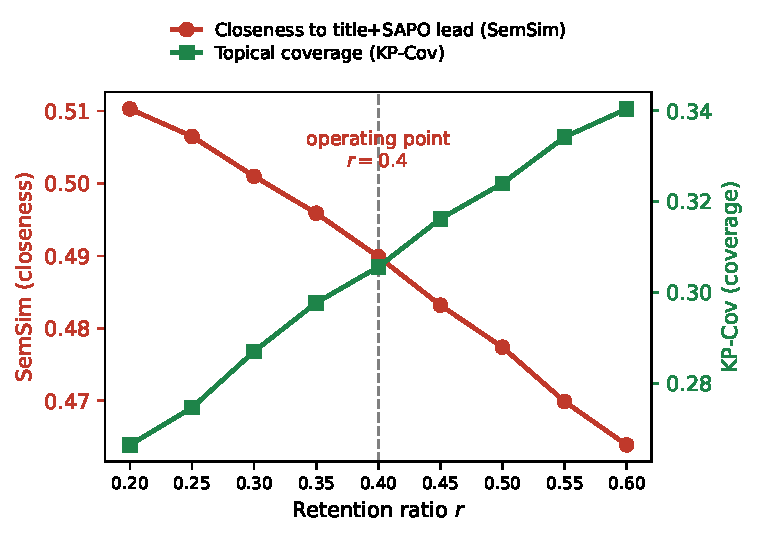
\includegraphics[width=0.92\columnwidth]{figures/retention_balance.pdf}
\caption{Đánh đổi theo tỉ lệ giữ câu $r$: độ gần lõi tiêu đề+sapo (SemSim, trục trái) giảm,
còn độ phủ chủ đề (KP-Cov, trục phải) tăng. Chúng tôi chọn $r{=}0{,}4$ làm điểm vận hành.}
\label{fig:retention}
\end{figure}

\subsection{Đánh giá trích xuất keyphrase (Tầng 2)}
Bảng~\ref{tab:keyphrase} cho thấy KeyBERT của StatLM dẫn đầu mọi độ đo. Khác biệt
giữa hai phiên bản KeyBERT (F1@10: 30,10 so với 25,51, cải thiện khoảng 18\%)
khẳng định vai trò của \emph{embedding bất đối xứng} trong việc thu hẹp khoảng
cách giữa keyphrase ngắn và tài liệu dài. WordAttractionRank dẫn đầu nhóm đồ thị
(F1@10 = 25,21) nhưng vẫn kém KeyBERT do mới dừng ở embedding mức từ và thiếu cơ
chế giảm trùng lặp như MMR.

\begin{table}[!t]
\renewcommand{\arraystretch}{1.2}
\caption{Kết quả đánh giá các phương pháp trích xuất keyphrase trên VietnamNet (đơn vị: \%)}
\label{tab:keyphrase}
\centering
\scriptsize
\setlength{\tabcolsep}{4pt}
\begin{tabular}{@{}lcccccc@{}}
\toprule
\textbf{Phương pháp} & \textbf{P@5} & \textbf{R@5} & \textbf{F1@5} & \textbf{P@10} & \textbf{R@10} & \textbf{F1@10} \\
\midrule
RAKE                       & 17,32 & 10,84 & 13,33 & 11,50 & 13,70 & 12,50 \\
YAKE                       & 20,15 & 12,67 & 15,56 & 14,45 & 17,50 & 15,83 \\
TextRank (từ khóa)         & 19,23 & 12,31 & 15,01 & 13,21 & 16,53 & 14,68 \\
TopicRank                  & 25,02 & 16,45 & 19,85 & 19,34 & 24,52 & 21,62 \\
Multipartite               & 26,83 & 17,67 & 21,31 & 20,47 & 26,26 & 23,01 \\
WordAttractionRank         & 28,49 & 17,43 & 21,63 & 23,16 & 27,66 & 25,21 \\
KeyBERT + emb. đối xứng     & 28,56 & 17,41 & 21,63 & 23,48 & 27,93 & 25,51 \\
\textbf{KeyBERT (StatLM)}  & \textbf{32,21} & \textbf{21,64} & \textbf{25,89} & \textbf{26,64} & \textbf{34,58} & \textbf{30,10} \\
\bottomrule
\end{tabular}
\end{table}

\subsection{Đánh giá không gian nhãn và phân loại (Tầng 3)}
Việc đánh giá không gian nhãn đòi hỏi cách tiếp cận hỗn hợp định lượng -- định
tính. Để bảo đảm tính khách quan khi phân loại thủ công 72 nhãn (26 của StatLM,
46 của X-MLClass-Gemini) vào năm nhóm, năm người đánh giá độc lập theo bộ hướng dẫn chuẩn
hóa. Độ nhất quán đo bằng Fleiss' $\kappa$ đạt $0{,}806$ (tỉ lệ đồng thuận thực
tế $\bar P\approx 0{,}866$, kỳ vọng ngẫu nhiên $\bar P_e\approx 0{,}307$), tương
ứng mức \emph{almost perfect} theo Landis \& Koch~\cite{landis1977}, xác nhận bộ
tiêu chí đủ tin cậy.

Bảng~\ref{tab:labelspace} so sánh cấu trúc không gian nhãn của hai hệ thống.
X-MLClass-Gemini làm việc trực tiếp trên chunk văn bản thô 50 token chứa nhiều tên riêng (``Hà
Nội'', ``VinFast'') và cụm meta báo chí (``Tin nóng 24h''); LLM không phân biệt
được chủ đề với thực thể/meta, dẫn đến 39,1\% nhãn nhiễu, đồng thời sinh 8 nhãn
đuôi dài nhưng vẫn bỏ trống 5 chuyên mục hẹp. Ngược lại, StatLM chủ động lọc
nhiễu từ hai tầng đầu: TextRank giữ câu trọng tâm, KeyBERT với lọc từ loại loại
bỏ thực thể/meta ngay khi trích keyphrase, khiến Gemini chỉ nhận 5 keyphrase sạch
và buộc phải khái quát hóa. Kết quả: không sinh Entity/Long-tail, tỉ lệ nhiễu chỉ
3,8\% và phủ 19/20 chuyên mục (gộp hợp lý các chuyên mục hẹp, ví dụ ``Bảo vệ
người tiêu dùng'' + ``Thị trường -- tiêu dùng'' $\rightarrow$ ``Tiêu dùng \& Thị
trường'').

\begin{table}[!t]
\renewcommand{\arraystretch}{1.2}
\caption{Cấu trúc và chất lượng không gian nhãn của X-MLClass-Gemini và StatLM}
\label{tab:labelspace}
\centering
\footnotesize
\begin{tabular}{@{}lcccc@{}}
\toprule
\multirow{2}{*}{\textbf{Nhóm nhãn}} & \multicolumn{2}{c}{\textbf{X-MLClass-Gemini}} & \multicolumn{2}{c}{\textbf{StatLM}} \\
\cmidrule(lr){2-3}\cmidrule(lr){4-5}
 & \textbf{SL} & \textbf{Tỉ lệ} & \textbf{SL} & \textbf{Tỉ lệ} \\
\midrule
Coarse      & 15 & 32,6\% & \textbf{20} & \textbf{76,9\%} \\
Long-tail   &  8 & 17,4\% &  0 &  0,0\% \\
Entity      &  6 & 13,0\% &  0 &  0,0\% \\
Meta/Noise  & 12 & 26,1\% &  1 &  3,8\% \\
Cross-topic &  5 & 10,9\% &  5 & 19,2\% \\
\midrule
\textbf{Tổng} & \textbf{46} & \textbf{100\%} & \textbf{26} & \textbf{100\%} \\
\midrule
Tỉ lệ nhiễu              & \multicolumn{2}{c}{39,1\%} & \multicolumn{2}{c}{\textbf{3,8\%}} \\
Chuyên mục phủ (Coarse)  & \multicolumn{2}{c}{15/20 (75\%)} & \multicolumn{2}{c}{\textbf{19/20 (95\%)}} \\
\bottomrule
\end{tabular}
\end{table}

Về khả năng gán nhãn đầu cuối, StatLM đạt $P@1=0{,}71$ và $P@3=0{,}84$, vượt xa
X-MLClass-Gemini ($P@1=0{,}49$, $P@3=0{,}63$). Nhờ 19/20 chuyên mục gốc đều có ít nhất một
nhãn Coarse tương ứng, hầu hết các bài đều có cơ hội được xếp hạng đúng ngay vị
trí 1; trong khi đó, 18 nhãn nhiễu (Entity + Meta/Noise) của X-MLClass-Gemini -- vốn không
phản ánh chủ đề -- thường chiếm mất rank 2--3 trên các bài giàu thực thể hoặc định
dạng báo chí, đẩy nhãn đúng xuống dưới.

\subsection{Đánh giá hiệu năng}
StatLM cũng nhanh hơn và rẻ hơn đáng kể. Nó giảm thời gian xử lý trung bình từ
$\sim$40 xuống $\sim$10 giây mỗi bài, giảm lượng token gửi đến LLM từ $\sim$900
xuống $\sim$30 mỗi bài (ít hơn khoảng 30 lần), và chỉ thực hiện 1 lần gọi API mỗi
bài thay vì $\sim$8 lần. Khác biệt đến từ việc StatLM chỉ gửi 5 keyphrase
($\sim$30 token) cho LLM, trong khi X-MLClass-Gemini gửi toàn bộ nội dung thô ($\sim$900
token/bài) và còn nhiều lần gọi API cho các bước phân cụm và xác minh trùng lặp.

\subsection{Phân tích ablation và thảo luận}
Bảng~\ref{tab:ablation} lượng hóa đóng góp của từng tầng (các giá trị có dấu
$\approx$ được ngoại suy theo xu hướng). Thay TextRank gốc bằng phiên bản embedding
giúp tỉ lệ coarse tăng 8--10\% và giảm nhiễu tương ứng. Bỏ Tầng~2 (gửi thẳng tóm
tắt cho LLM) khiến tỉ lệ coarse giảm mạnh từ 76,9\% xuống $\approx$55\% -- cho
thấy keyphrase là cầu nối then chốt giữa tóm tắt và LLM. Thay Tầng~2 bằng embedding
đối xứng làm F1@10 giảm khoảng 15\% và kéo nhiễu nhãn tăng gần gấp đôi. Những quan
sát này khẳng định thiết kế ``làm sạch trước, khái quát sau'' là hợp lý và từng
thành phần đều khó thay thế.

\begin{table}[!t]
\renewcommand{\arraystretch}{1.25}
\caption{Ảnh hưởng của từng tầng đến chất lượng không gian nhãn cuối cùng
(T1: ROUGE-1 F1; T2: F1@10; T3: Coarse / Nhiễu / Số chuyên mục được phủ).}
\label{tab:ablation}
\centering
\footnotesize
\begin{tabularx}{\columnwidth}{@{}Xcc>{\raggedright\arraybackslash}X@{}}
\toprule
\textbf{Biến thể} & \textbf{T1} & \textbf{T2} & \textbf{T3 (Coarse/Nhiễu/Phủ)} \\
\midrule
StatLM đầy đủ          & 0,403 & 30,10 & 76,9\% / 3,8\% / 19/20 \\
T1 $\to$ TextRank gốc  & 0,341 & $\approx$28,5 & $\approx$68\% / $\approx$10\% / 17/20 \\
Bỏ T1                  & --    & $\approx$27,0 & $\approx$65\% / $\approx$15\% / 16/20 \\
T2 $\to$ đối xứng       & 0,403 & 25,51 & $\approx$70\% / $\approx$8\% / 17/20 \\
Bỏ T2                  & 0,403 & --    & $\approx$55\% / $\approx$20\% / 14/20 \\
\bottomrule
\end{tabularx}
\end{table}

Bức tranh tổng thể làm nổi bật triết lý \emph{Statistical Encoder -- Language
Model Decoder}. X-MLClass-Gemini dù kế thừa sức mạnh của pipeline gốc vẫn bộc lộ điểm yếu khi
gặp dữ liệu báo chí thực tế: LLM bị phân tán bởi thực thể và cụm định dạng, tạo
không gian nhãn nhiễu và tốn kém. StatLM giải quyết một cách hệ thống bằng cách
chủ động lọc nhiễu trước khi dữ liệu đến LLM, cho ra không gian nhãn gọn, sạch,
tập trung vào nhãn thô (Coarse), đồng thời giảm mạnh chi phí token và thời gian.
Nói cách khác, để có một bộ nhãn thô hữu ích, một chiến lược ``làm sạch trước,
khái quát sau'' đơn giản và tiết kiệm như StatLM là đủ dùng, không cần đến một
pipeline phức tạp và đắt đỏ. Kết quả ablation (Bảng~\ref{tab:ablation}) còn cho
thấy hai tầng encoder bổ trợ chứ không thay thế lẫn nhau: Tầng~1 nâng chất lượng
đầu vào của Tầng~2, còn embedding bất đối xứng ở Tầng~2 là điều kiện cần để LLM
nhận được keyphrase đủ sạch -- cả hai cùng quyết định độ tinh gọn của không gian
nhãn cuối cùng.

